% !TEX program = xelatex
\documentclass[UTF8,fontset=fandol,a4paper,11pt]{ctexart}
\usepackage[margin=21mm,top=23mm,bottom=22mm,headheight=16pt]{geometry}
\usepackage{amsmath,amssymb,mathtools,bm}
\usepackage{tikz}
\usetikzlibrary{arrows.meta,calc,angles,quotes,patterns}
\usepackage{xcolor,booktabs,array,longtable,enumitem,fancyhdr,needspace}
\usepackage[unicode,hidelinks]{hyperref}
\definecolor{ink}{HTML}{24343C}
\definecolor{accent}{HTML}{166A70}
\definecolor{muted}{HTML}{65747A}
\definecolor{rulegray}{HTML}{D4DDE0}
\definecolor{warm}{HTML}{966037}
\color{ink}
\setlength{\parindent}{2em}
\setlength{\parskip}{4pt}
\linespread{1.12}
\AtBeginDocument{\setlength{\abovedisplayskip}{6pt plus 2pt minus 1pt}
\setlength{\belowdisplayskip}{6pt plus 2pt minus 1pt}
\setlength{\abovedisplayshortskip}{0pt plus 1pt}
\setlength{\belowdisplayshortskip}{4pt plus 1pt}}
\setlist[enumerate]{label=(\arabic*),leftmargin=2.3em,itemsep=3pt,topsep=4pt}
\setlist[itemize]{leftmargin=2em,itemsep=2pt,topsep=4pt}
\allowdisplaybreaks[1]
\setlength{\emergencystretch}{2em}
\setcounter{secnumdepth}{0}
\providecommand{\tightlist}{\setlength{\itemsep}{0pt}\setlength{\parskip}{0pt}}
\ctexset{section={format=\Large\bfseries\color{accent},beforeskip=10pt,afterskip=9pt},
subsection={format=\normalsize\bfseries\color{accent},beforeskip=10pt,afterskip=4pt},
subsubsection={format=\normalsize\bfseries,beforeskip=8pt,afterskip=3pt}}
\pagestyle{fancy}
\fancyhf{}
\fancyhead[L]{\small\color{muted}物理学难题集萃}
% 页眉仅保留书名；版本名称只在封面显示。
\fancyfoot[L]{\small\color{muted}\chapterlabel}
\fancyfoot[R]{\small\thepage}
\renewcommand{\headrulewidth}{0.4pt}
\renewcommand{\footrulewidth}{0pt}
\newcommand{\dd}{\mathop{}\!\mathrm{d}}
\newcommand{\vect}[1]{\bm{#1}}
\newcommand{\tagline}[1]{\noindent{\small\color{muted}#1}\par}
\newcommand{\result}[1]{\begin{equation*}\boxed{#1}\end{equation*}}
\newcommand{\figcaption}[1]{\par\vspace{2pt}{\small\color{muted}#1}\par}
\newcommand{\teach}[2]{\Needspace{4\baselineskip}\subsection*{讲解要点与追问}#1\par\smallskip\noindent\textbf{追问：}#2\par}
\newcommand{\workarea}{\par\vspace{7mm}\noindent{\small\color{muted}作答区}\par\vspace{4mm}
\noindent\textcolor{rulegray}{\rule{\linewidth}{0.3pt}}\par\vspace{16mm}
\noindent\textcolor{rulegray}{\rule{\linewidth}{0.3pt}}\par\vspace{16mm}
\noindent\textcolor{rulegray}{\rule{\linewidth}{0.3pt}}\par\vspace{16mm}
\noindent\textcolor{rulegray}{\rule{\linewidth}{0.3pt}}}
\tikzset{axis/.style={-{Stealth[length=2mm]},thin,color=muted},
motion/.style={-{Stealth[length=2.3mm]},thick,color=accent},
force/.style={-{Stealth[length=2.3mm]},thick,color=warm},
traj/.style={thick,color=accent},guide/.style={dashed,thin,color=muted},
object/.style={thick,color=ink},every node/.style={font=\small}}\widowpenalty=10000\clubpenalty=10000\displaywidowpenalty=10000\newcommand{\chapterlabel}{电磁学试题（一）}







\hypersetup{pdftitle={电磁学试题（一）·学生版},pdfauthor={}}

\begin{document}\pdfbookmark[0]{电磁学试题（一）}{cover}

\thispagestyle{empty}\vspace*{22mm}

\noindent{\Huge\bfseries 物理学难题集萃}\par\vspace{12mm}

\noindent{\LARGE 电磁学试题（一）}\par\vspace{12mm}

\noindent{\Large\color{accent}学生版}\par\vspace{9mm}

\noindent\textcolor{accent}{\rule{\linewidth}{1pt}}\par\vspace{9mm}

\noindent 第1--5题\par\vfill\clearpage

\pdfbookmark[1]{题目目录}{contents}\section*{题目目录}

\begin{longtable}{@{}r p{113mm} r@{}}\toprule 题号 & 题目 & 页码\\\midrule

\hyperref[q:1]{1} & \hyperref[q:1]{均匀电场中弹簧两端的带电小球} & \pageref{q:1} \\

\hyperref[q:2]{2} & \hyperref[q:2]{半无限导线向平面径向分流的磁场} & \pageref{q:2} \\

\hyperref[q:3]{3} & \hyperref[q:3]{水平磁场中下落带电球的临界轨迹} & \pageref{q:3} \\

\hyperref[q:4]{4} & \hyperref[q:4]{弱磁场中异号带电双体的质心摆线} & \pageref{q:4} \\

\hyperref[q:5]{5} & \hyperref[q:5]{带电容滑动双棒的充电与最终速度} & \pageref{q:5} \\

\bottomrule\end{longtable}

\clearpage

\pdfbookmark[2]{第 1 题 均匀电场中弹簧两端的带电小球}{q1}

\section*{第 1 题\quad 均匀电场中弹簧两端的带电小球}\label{q:1}


自由长度为$L$、劲度系数为$k$的轻弹簧，两端连接小球1、2，质量分别为$m_1,m_2$，正电荷分别为$Q_1,Q_2$。两球处于均匀电场中，场强$\boldsymbol E=E\hat x$沿初始连线由球1指向球2。初始两球静止、弹簧为自由长度。忽略重力、两球之间的电相互作用及辐射。
求此后两球间的最大距离，给出运动方程并讨论参数的不同情形。$L$足够大，保证压缩时两球始终不相碰、左右次序不交换。


\begin{center}\begin{minipage}{.98\linewidth}\centering
\begin{tikzpicture}[scale=.9,transform shape]

\draw[object] (.5,0)--(1,0)--(1.15,.2)--(1.45,-.2)--(1.75,.2)--(2.05,-.2)--(2.35,.2)--(2.65,-.2)--(2.95,.2)--(3.25,-.2)--(3.55,.2)--(3.85,-.2)--(4.15,.2)--(4.3,0)--(5,0);
\fill[accent!12] (.5,0) circle (.15);\draw[object] (.5,0) circle (.15);
\fill[warm!12] (5,0) circle (.15);\draw[object] (5,0) circle (.15);
\node[below,align=center] at (.5,-.3) {球1\\$m_1,Q_1$};
\node[below,align=center] at (5,-.3) {球2\\$m_2,Q_2$};
\draw[axis,<->] (.5,-1.9)--(5,-1.9) node[midway,below] {初始 $r=L$};
\draw[force] (1.3,1)--(4.2,1) node[midway,above] {$\boldsymbol E=E\hat x$};
\node at (2.7,.4) {$k$};

\end{tikzpicture}
\figcaption{图电试1.1\quad 初始弹簧为自由长度，电场由球1指向球2。}
\end{minipage}\end{center}

\workarea

\clearpage

\pdfbookmark[2]{第 2 题 半无限导线向平面径向分流的磁场}{q2}

\section*{第 2 题\quad 半无限导线向平面径向分流的磁场}\label{q:2}


稳恒电流$I$沿负$x$半轴流向原点$O$，到达$x=0$的无限大平面后均匀向各径向散开。平面上的面电流密度为
\[
\boldsymbol K(\rho)=\frac{I}{2\pi\rho}\hat{\boldsymbol\rho},\qquad \rho>0.
\]
求右半空间$x>0$、左半空间$x<0$以及平面两侧的磁场。规定$\hat{\boldsymbol\phi}$绕$+x$轴按右手方向，真空磁导率为$\mu_0$。另说明理想电流面上以及理想细导线轴线上的场应怎样理解。


\begin{center}\begin{minipage}{.98\linewidth}\centering
\begin{tikzpicture}[scale=.9,transform shape]

\fill[accent!5] (0,-1.7)--(1.8,-.7)--(1.8,2.7)--(0,1.7)--cycle;
\draw[object] (0,-1.7)--(1.8,-.7)--(1.8,2.7)--(0,1.7)--cycle;
\coordinate (O) at (.9,.5);
\draw[object] (-3,.5)--(O);
\draw[motion] (-2.3,.5)--(-.8,.5) node[midway,above] {$I$};
\foreach \ang in {20,80,140,200,260,320}{
\draw[motion] (O)--({.9+.7*cos(\ang)},{.5+1.45*sin(\ang)});}
\draw[axis] (O)--(4,.5) node[right] {$+x$};
\fill (O) circle (1.6pt) node[below right] {$O$};
\node at (.9,3.1) {$x=0$，无限径向分流面};
\node at (1,-2.4) {$K_\rho=I/(2\pi\rho)$};

\end{tikzpicture}
\figcaption{图电试1.2\quad 轴向电流在O转为面内径向电流，构型绕x轴对称。}
\end{minipage}\end{center}

\par\vspace{5mm}\noindent{\small\color{muted}作答区}\par\vspace{3mm}\noindent\textcolor{rulegray}{\rule{\linewidth}{0.3pt}}\par\vspace{12mm}\noindent\textcolor{rulegray}{\rule{\linewidth}{0.3pt}}

\clearpage

\pdfbookmark[2]{第 3 题 水平磁场中下落带电球的临界轨迹}{q3}

\section*{第 3 题\quad 水平磁场中下落带电球的临界轨迹}\label{q:3}


质量$m$、正电荷$q$的小球在离水平地面高度$h$处由静止开始运动，只受重力和匀强磁场的洛伦兹力。磁场水平，空气阻力、辐射忽略，$g$为常量。
求使小球始终不接触地面的磁感应强度条件，给出临界场值及其轨迹，并说明“严格不接触”时是否存在可取得的最小磁场。
取$x$向右、$y$竖直向下，原点为初始位置，磁场沿$\hat x\times\hat y$方向。


\begin{center}\begin{minipage}{.98\linewidth}\centering
\begin{tikzpicture}[scale=.9,transform shape]

\draw[axis] (0,0)--(5,0) node[right] {$x$};
\draw[axis] (0,0)--(0,-3.7) node[below] {$y$};
\draw[object] (-.5,-3)--(5,-3);
\fill[muted!15] (-.5,-3) rectangle (5,-3.2);
\fill[accent] (0,0) circle (2pt) node[above left] {$O:\ m,q$};
\draw[force] (.4,-.1)--(.4,-1) node[right] {$mg$};
\draw[axis,<->] (4.4,0)--(4.4,-3) node[midway,right] {$h$};
\node at (2.6,-.7) {$\otimes\ \boldsymbol B$};
\node at (2.8,-2.6) {地面 $y=h$};

\end{tikzpicture}
\figcaption{图电试1.3\quad 坐标y向下，磁场指向纸内；初始速度为零。}
\end{minipage}\end{center}

\workarea

\clearpage

\pdfbookmark[2]{第 4 题 弱磁场中异号带电双体的质心摆线}{q4}

\section*{第 4 题\quad 弱磁场中异号带电双体的质心摆线}\label{q:4}


质量均为$m$、电荷分别为$+q$与$-q$的两质点相距$2R$。以其质心$C$为原点，取$x$向右、$y$向上。$t=0$时$+q$在$(0,-R)$、$-q$在$(0,R)$，两者速度构成绕$C$顺时针的半径$R$圆运动，质心初速为零。初始圆运动角频率$\omega$由库仑引力确定。
考察这一初态在沿$+z$的弱匀强静磁场$\boldsymbol B=B\hat z$中的后续运动；忽略重力、辐射及建场过程的感应冲量。取$qB/(m\omega)\ll1$，只求关于$B$的一阶质心运动，近似保持内部圆运动不变。
\begin{enumerate}
\item 求$v_{Cx}(t),v_{Cy}(t)$。
\item 求$X_C(t),Y_C(t)$并画轨迹。
\item 说明这一近似为何不与磁力不做功、系统能量守恒矛盾。
\end{enumerate}


\begin{center}\begin{minipage}{.98\linewidth}\centering
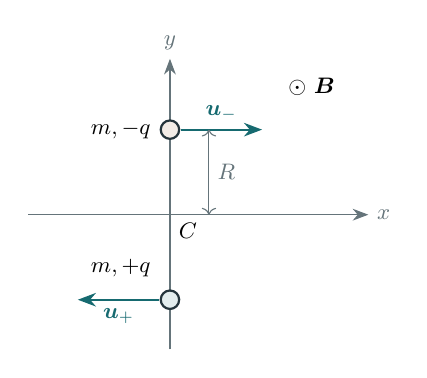
\begin{tikzpicture}[scale=.9,transform shape]

\draw[axis] (-2,0)--(2.8,0) node[right] {$x$};
\draw[axis] (0,-1.9)--(0,2.2) node[above] {$y$};
\fill[accent!12] (0,-1.2) circle (.13);\draw[object] (0,-1.2) circle (.13);
\fill[warm!12] (0,1.2) circle (.13);\draw[object] (0,1.2) circle (.13);
\node[left] at (-.15,1.2) {$m,-q$};\node[above left] at (-.15,-1) {$m,+q$};
\draw[motion] (.15,1.2)--(1.3,1.2) node[midway,above] {$\boldsymbol u_-$};
\draw[motion] (-.15,-1.2)--(-1.3,-1.2) node[midway,below] {$\boldsymbol u_+$};
\node[below right] at (0,0) {$C$};
\node at (2,1.8) {$\odot\ \boldsymbol B$};
\draw[axis,<->] (.55,0)--(.55,1.2) node[midway,right] {$R$};

\end{tikzpicture}
\figcaption{图电试1.4\quad 上方负电荷向右、下方正电荷向左，初始内部运动顺时针。}
\end{minipage}\end{center}

\par\vspace{5mm}\noindent{\small\color{muted}作答区}\par\vspace{3mm}\noindent\textcolor{rulegray}{\rule{\linewidth}{0.3pt}}\par\vspace{12mm}\noindent\textcolor{rulegray}{\rule{\linewidth}{0.3pt}}

\clearpage

\pdfbookmark[2]{第 5 题 带电容滑动双棒的充电与最终速度}{q5}

\section*{第 5 题\quad 带电容滑动双棒的充电与最终速度}\label{q:5}


两条水平、足够长的平行导轨上有左右两根可无摩擦滑动的导体棒。每根棒长度$l$、质量$m$、电阻$R$，棒中各串接一个电容为$C$的相同电容器，两个电容器初始均未充电；导轨电阻可忽略，组成矩形回路。均匀静磁场$B$垂直回路平面向内。初始左棒静止，右棒以$v_0>0$沿导轨向右运动，初始棒间距$d_0$有限，所有辐射与回路自感忽略。
\begin{enumerate}
\item 对电容$C$的充电过程，能否用静止回路等效：保持两棒的电阻$R$及两电容$C$，再串联一个电容$C'$与恒定电源$\mathcal E'$，于$t=0$闭合？若能，求$\mathcal E',C'$。
\item 求两棒速度、电容电荷随时间的关系。
\item 求两棒最终速度，说明是否相等；带电容时棒间距是否趋向有限值？
\item 将两个电容器取去、用导线接通相应断点，求此时最终速度和棒间距的极限。
\end{enumerate}


\begin{center}\begin{minipage}{.98\linewidth}\centering
\begin{tikzpicture}[scale=.9,transform shape]

\draw[object] (-.6,0)--(5,0);\draw[object] (-.6,2.7)--(5,2.7);
\foreach \x in {0,4}{
\draw[object] (\x,0)--(\x,.95);
\draw[object,line width=1pt] (\x-.36,.95)--(\x+.36,.95);
\draw[object,line width=1pt] (\x-.36,1.15)--(\x+.36,1.15);
\draw[object] (\x,1.15)--(\x,1.8);
\draw[object] (\x-.14,1.8) rectangle (\x+.14,2.35);
\draw[object] (\x,2.35)--(\x,2.7);
\node[right] at (\x+.5,1.05) {$C$};
\node[right] at (\x+.2,2.08) {$R$};
}
\node at (2,1.6) {$\otimes\ B$};
\draw[axis,<->] (-.9,0)--(-.9,2.7) node[midway,left] {$l$};
\draw[motion] (4.15,3.2)--(5.4,3.2) node[midway,above] {$v_0$};
\node[above] at (0,3) {初始静止};
\draw[axis,<->] (0,-.5)--(4,-.5) node[midway,below] {$d_0$};

\end{tikzpicture}
\figcaption{图电试1.5\quad 两棒各串一个C、各有电阻R；初始电容均不带电。}
\end{minipage}\end{center}

\par\vspace{5mm}\noindent{\small\color{muted}作答区}\par\vspace{3mm}\noindent\textcolor{rulegray}{\rule{\linewidth}{0.3pt}}\par\vspace{12mm}\noindent\textcolor{rulegray}{\rule{\linewidth}{0.3pt}}

\end{document}
